%!TEX root = ../template.tex
%%%%%%%%%%%%%%%%%%%%%%%%%%%%%%%%%%%%%%%%%%%%%%%%%%%%%%%%%%%%%%%%%%%%
%% chapter2.tex
%% NOVA thesis document file
%%
%% Chapter with the template manual
%%%%%%%%%%%%%%%%%%%%%%%%%%%%%%%%%%%%%%%%%%%%%%%%%%%%%%%%%%%%%%%%%%%%

\typeout{NT FILE chapter2.tex}%
\glsresetall
\

\chapter{Related Work}
\label{cha:related_work}

With the objective of understanding the current state of the art in the field of \gls{VR} 
navigation and locomotion, this chapter presents several topics, techniques and studies that are relevant to this field.

\section{Virtual Reality}
\label{sec:vr-background}

\gls{VR} has been given various definitions\cite{Mazuryk1999}, but these tend to converge on the same few essential ideas: It is a real-time,
interactive and immersive experience in a simulated 3D World (commonly referred as \glspl{VE}), made possible through the use of different technologies, 
as \glspl{HMD} and several input/tracking devices that have been in active development and research as of late \cite{Boletsis2022}.

It's through the understanding and right application of these technologies and research that a \gls{VR} application can realize its full 
immersive potential \cite{Lee2020}. Recognizing that this is one of the key points in \gls{VR} development \cite{Schwind2019}, 
this section is dedicated to the exploration of said literature and technologies.

\subsection{Head-Mounted Displays and Devices}
\label{sec:hmds-devices}

The start in development of consumer accessible \glspl{HMD} in 2012 can be considered the initial spark of the denominated second-wave of \gls{VR} 
development, greatly contributing to research in the field of \gls{HCI} \cite{Anthes2016}. This wave of development is still underway and with it 
new devices are being introduced into the market \cite{Lee2020}.

\glspl{HMD} consist of two screens mounted in a glasses-like device that are fixed relative to
the wearer's eye position, and portray the \gls{VE} by obtaining the user's head
orientation and position from a tracking system \cite{Santos2009}. 
Tracking Systems are, therefore, technologies that permit the correct tracking 
of the wearer's head movements according to the \gls{6DOF} \cite{Anthes2016} - \textbf{Surge}, \textbf{Sway} and \textbf{Heave} 
- translational movements in the x, y and z axis, respectively 
- and \textbf{Pitch}, \textbf{Yaw} and \textbf{Roll} - rotational movements in the x, y and z axis, respectively.

According to Anthes et. al \cite{Anthes2016}, \glspl{HMD} can also be divided into two different categories:

\begin{itemize}

    \item Wired \glspl{HMD} - These devices need to be connected to a powerful \gls{PC} in order to funtion. 
    The differences between the devices of this type range from the screen's resolution, \gls{FOV}, weight, as well as 
    additional features such as cameras that permit \gls{AR} capabilities and eye tracking systems to record the users gaze.
    They are typically empowered by the \gls{6DOF} tracking system provided by the manufacturer of the \gls{HMD}. 

    \item Mobile \glspl{HMD} - These range from \glspl{HMD} with a computing system within the headset to frames and cases for 
    smartphones with additional lenses, but all share the property of not being dependent on an external \gls{PC}.
    Wired \glspl{HMD} tend to have better specifications, but later developments of \glspl{HMD} like the Oculus Quest 3
    \footnote{Oculus Quest 3 Information Page - \href{https://www.meta.com/quest/quest-3/}{https://www.meta.com/quest/quest-3/}, Last Access - Jan 2025 } have 
    changed this perspective, by providing competent display specifications and pairing it with high resolution cameras and sensors, such as 
    gyroscopes, accelerometers and magnetometers for tracking systems that allow wireless \gls{6DOF} and Gesture Tracking (Figure~\ref{fig:hmd-quest}).
\end{itemize}

\begin{figure}[b]
    \centering
    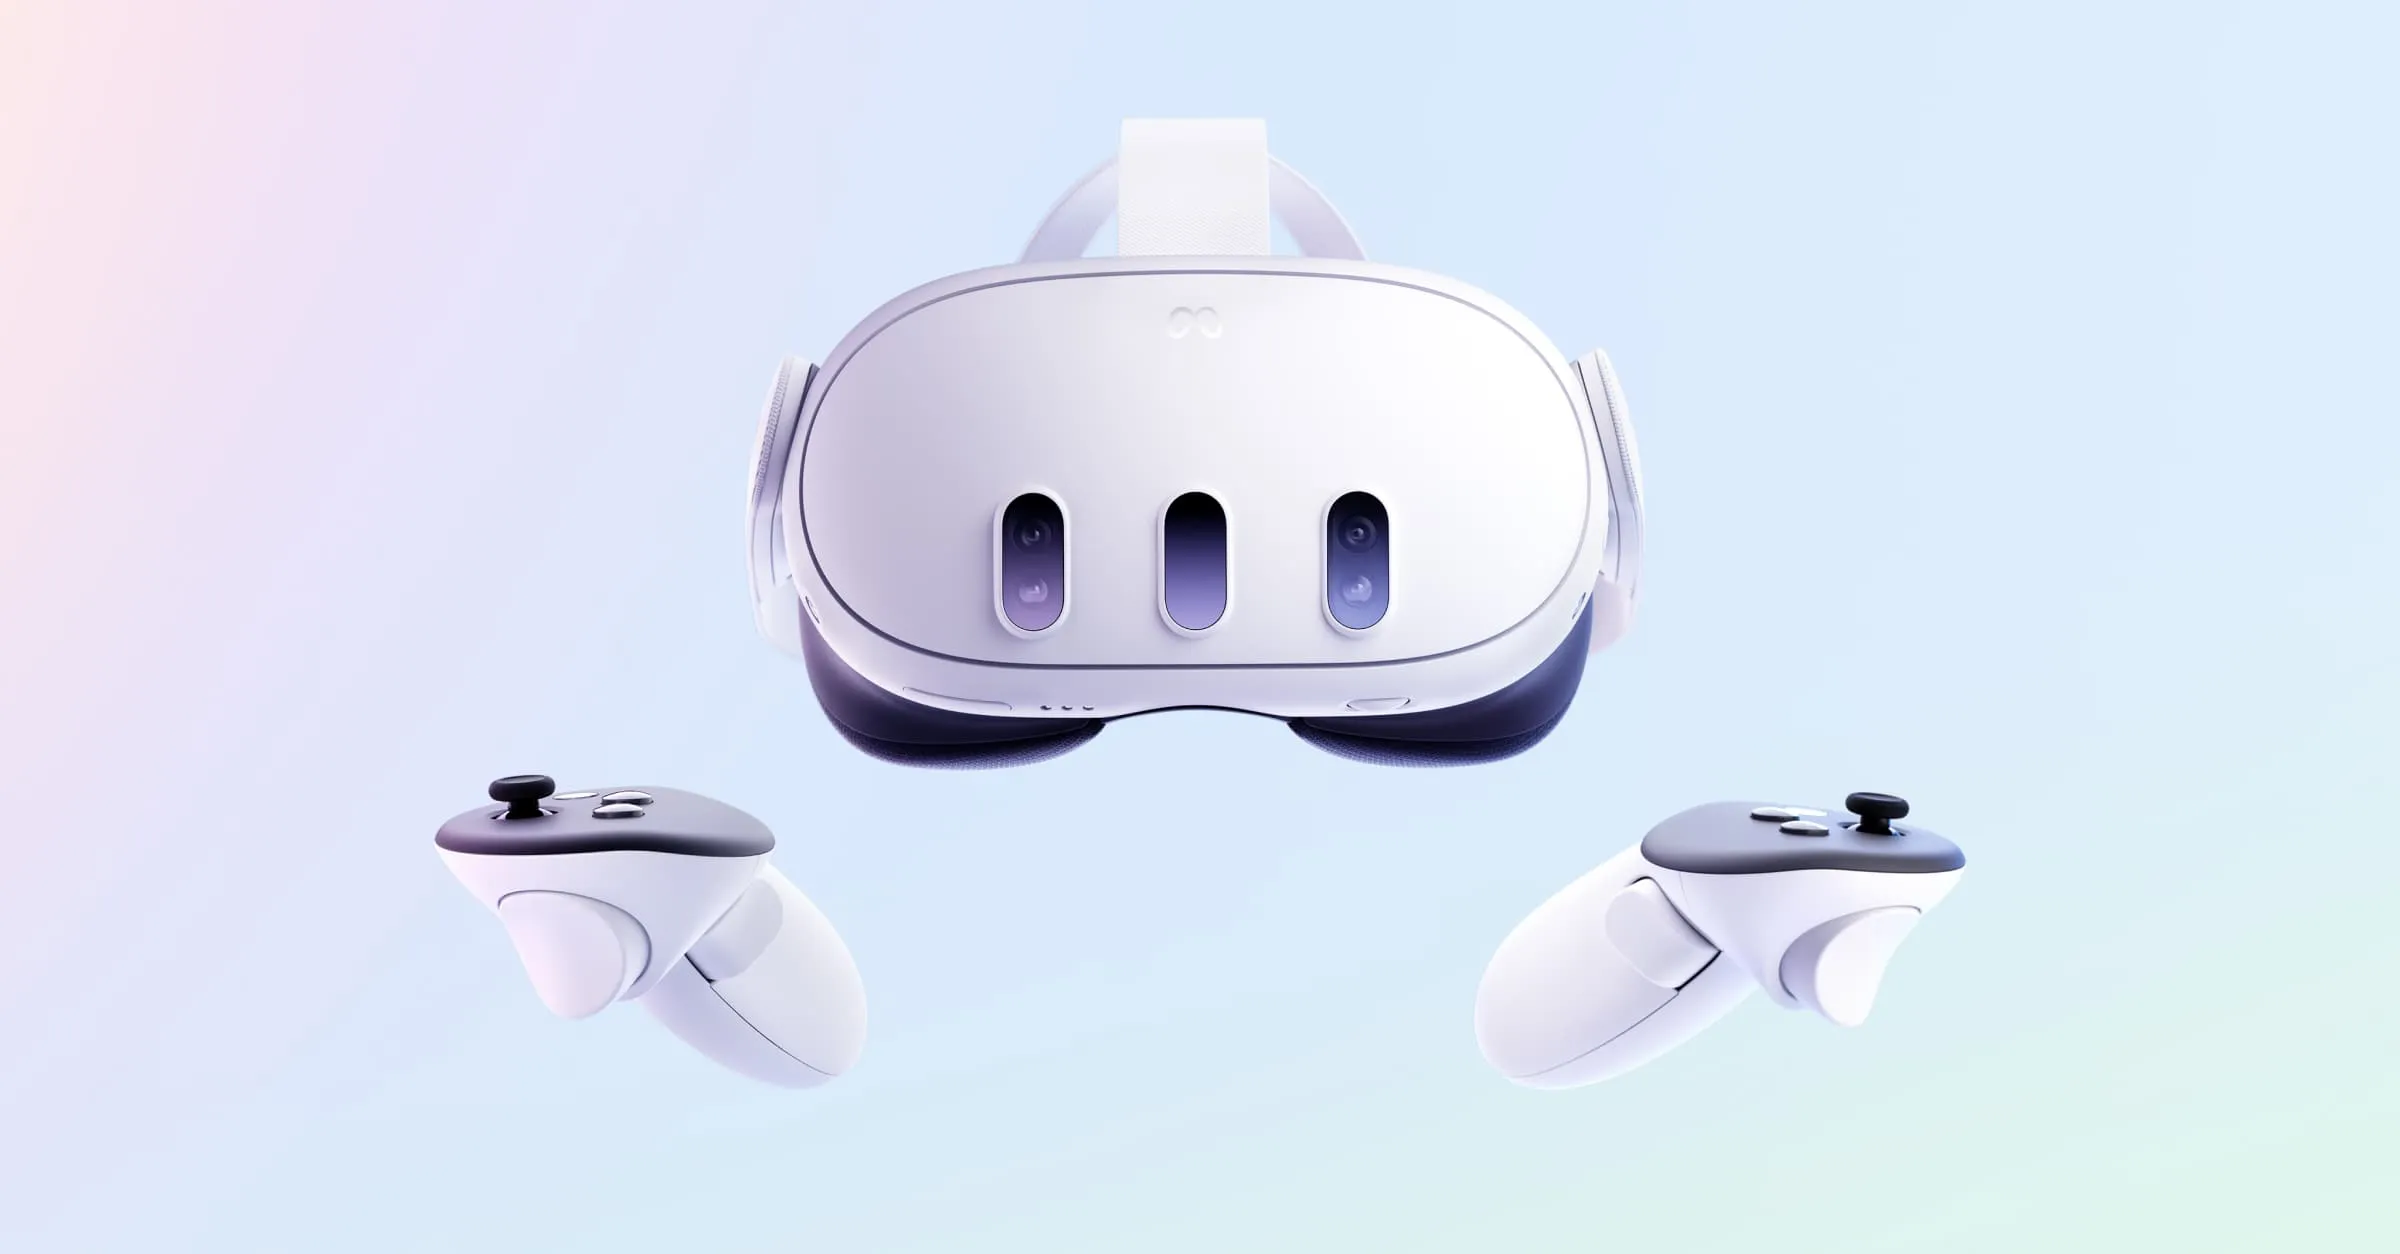
\includegraphics[width=0.8\textwidth]{NOVAthesisFiles/Images/papers/hmd-quest.png}
    \caption{The Oculus Quest 3 and its Controllers. The headset's frontal cameras and IMU(Inertial Measurement Unit) allow a wireless 
    \gls{6DOF} and gesture tracking system.}
    \label{fig:hmd-quest}
\end{figure}

Input devices also have their importance in users' interactions with \glspl{VE} \cite{Lee2020}, with these taking multiple forms.
Controllers are the most common within the \gls{VR} space \cite{Anthes2016,Boletsis2022}, demonstrating similarities with the familiar 
video-game controllers with the inclusions of buttons for discrete input, and joysticks and triggers for continuous input. \gls{VR} controllers 
distinguish themselves from the video game ones by including \gls{6DOF} tracking capabilities and by integrating gesture-recognizing sensors.

Other input devices range from Gesture Tracking devices, with data gloves as an example, to Navigation Devices, such as \glspl{ODT} 
and Zero-Friction Surfaces \cite{Anthes2016,Nilsson2018}.

\subsection{Navigation of Virtual Environments}
\label{sec:navigation-in-ves}

Due to the immersive yet controlled nature of \gls{VR}, one of its effective applications involves the study of human navigation behavior 
\cite{Feng2022}. This research belongs with those studies, thus it's relevant to have an overview on this matter, as well as understanding its 
nomenclature, which is the objective of this section.

\textbf{Navigation} can be broken down into \textit{Motion} - its physical element - and \textit{Wayfinding} - its cognitive element 
\cite{Eastgate2014}. The model constructed by Jul and Furnas \cite{Jul1997}, as seen on Figure\ref{fig:nav-model} is considered a relatively complete representation 
of how Navigation takes place, since it takes both these elements into consideration.

 \begin{figure}[b]
    \centering
    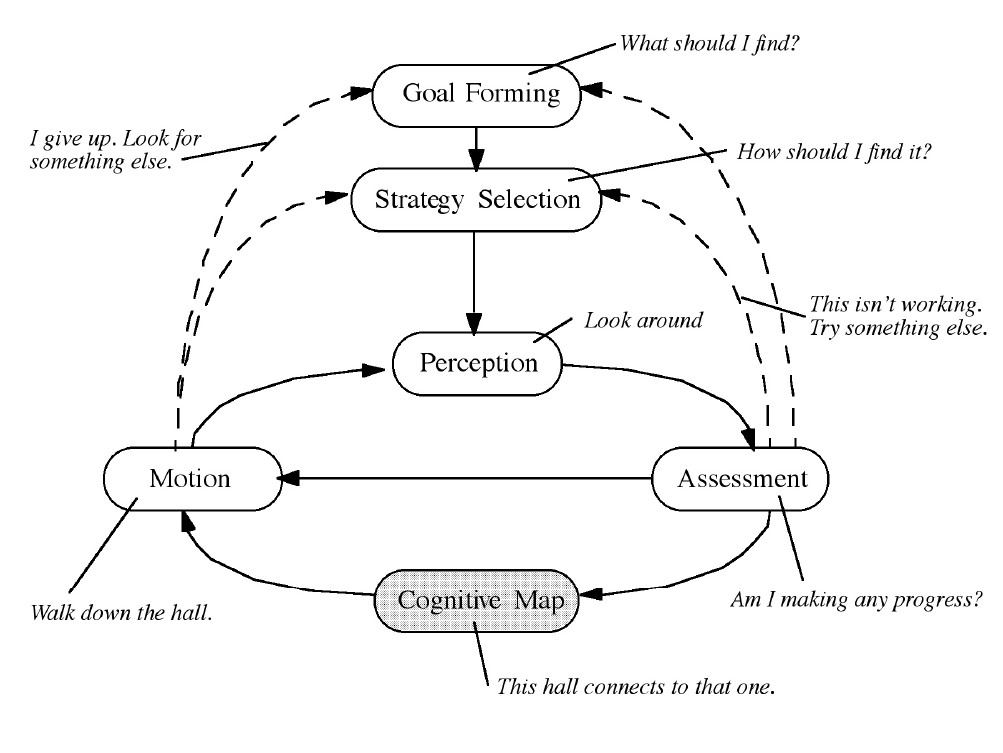
\includegraphics[width=0.6\textwidth]{NOVAthesisFiles/Images/papers/nav-model.png}
    \caption{Model by Jul and Furnas that demonstrates the motor and cognitive elements of Navigation \cite{Eastgate2014}.}
    \label{fig:nav-model}
\end{figure}

\textit{Wayfinding} involves no movement of any kind, and its primary purpose is to construct and keep a \textit{cognitive map}
 \cite{Langbehn2018}, also referred to as \textit{mental maps}, which, as the name suggests, is a mental representation of an environment. 
 Although it may be instinctive to call it a "picture in our heads", studies have come to suggest that these cognitive representations 
 aren't strictly visual but also symbolic \cite{Eastgate2014, Warren2019}. A \textit{cognitive map's} "quality" is then dependent on the 
 method in which the spatial knowledge is acquired, as results of accurate spatial orientation differs from understanding a map to navigating  
 non-immersive \glspl{VE} (like those of video-games on a screen) and immersive \glspl{VE} \cite{Eastgate2014,Santos2009}. Even then these 
 results can be inconclusive, as the properties of \glspl{VE} affect the intake of spatial knowledge.

\textit{Motion}, also referred as \textit{Locomotion} or \textit{Travel}, being the motor element of Navigation that allows the physical translation 
from on location to another \cite{Santos2009}. The properties of motion have implications on the intake of spatial knowledge, as for instance, 
if locomotion in a \gls{VE} is discrete instead of continuous, users tend to have more difficulty in fully comprehending their surroundings. This 
and other properties of locomotion are then going to be discussed in the following sections of \nameref{sec:vr-locomotion-techniques} and 
\nameref{sec:non-euclidean-space}.

\section{VR Locomotion Techniques}
\label{sec:vr-locomotion-techniques}

Locomotion (also denoted as "active travel" or just "travel"\cite{Langbehn2018}) - 
the act of moving from one location to another - is often considered one of the key aspects of \gls{VR} interaction\cite{8255772}, 
as it permits navigation in \glspl{VE} \cite{Boletsis2019}.

Throughout the advancements in \gls{VR} research and technology, multiple locomotion techniques have been developed, 
all with different characteristics, addressing different needs and use cases\cite{Boletsis2022}. 
It's due to the diversity of these techniques that various typonomies and classifications have been proposed,
throughout the years of \gls{VR} development \cite{Boletsis2022}. 
The structure of this subsection is based on the typology of \gls{VR} Locomotion Techniques proposed by Boletsis et al. 
\cite{Boletsis2022} as it encompasses most techniques according to the characteristics discussed in this section.

According with Boletsis et al. \cite{Boletsis2022} locomotion techniques are distinguished by the type of interaction they require, 
the type of motion it produces and the type of \gls{VE} it is designed for, as seen in Figure~\ref{fig:vr-locomotion-typology}.

\begin{figure}[b]
    \centering
    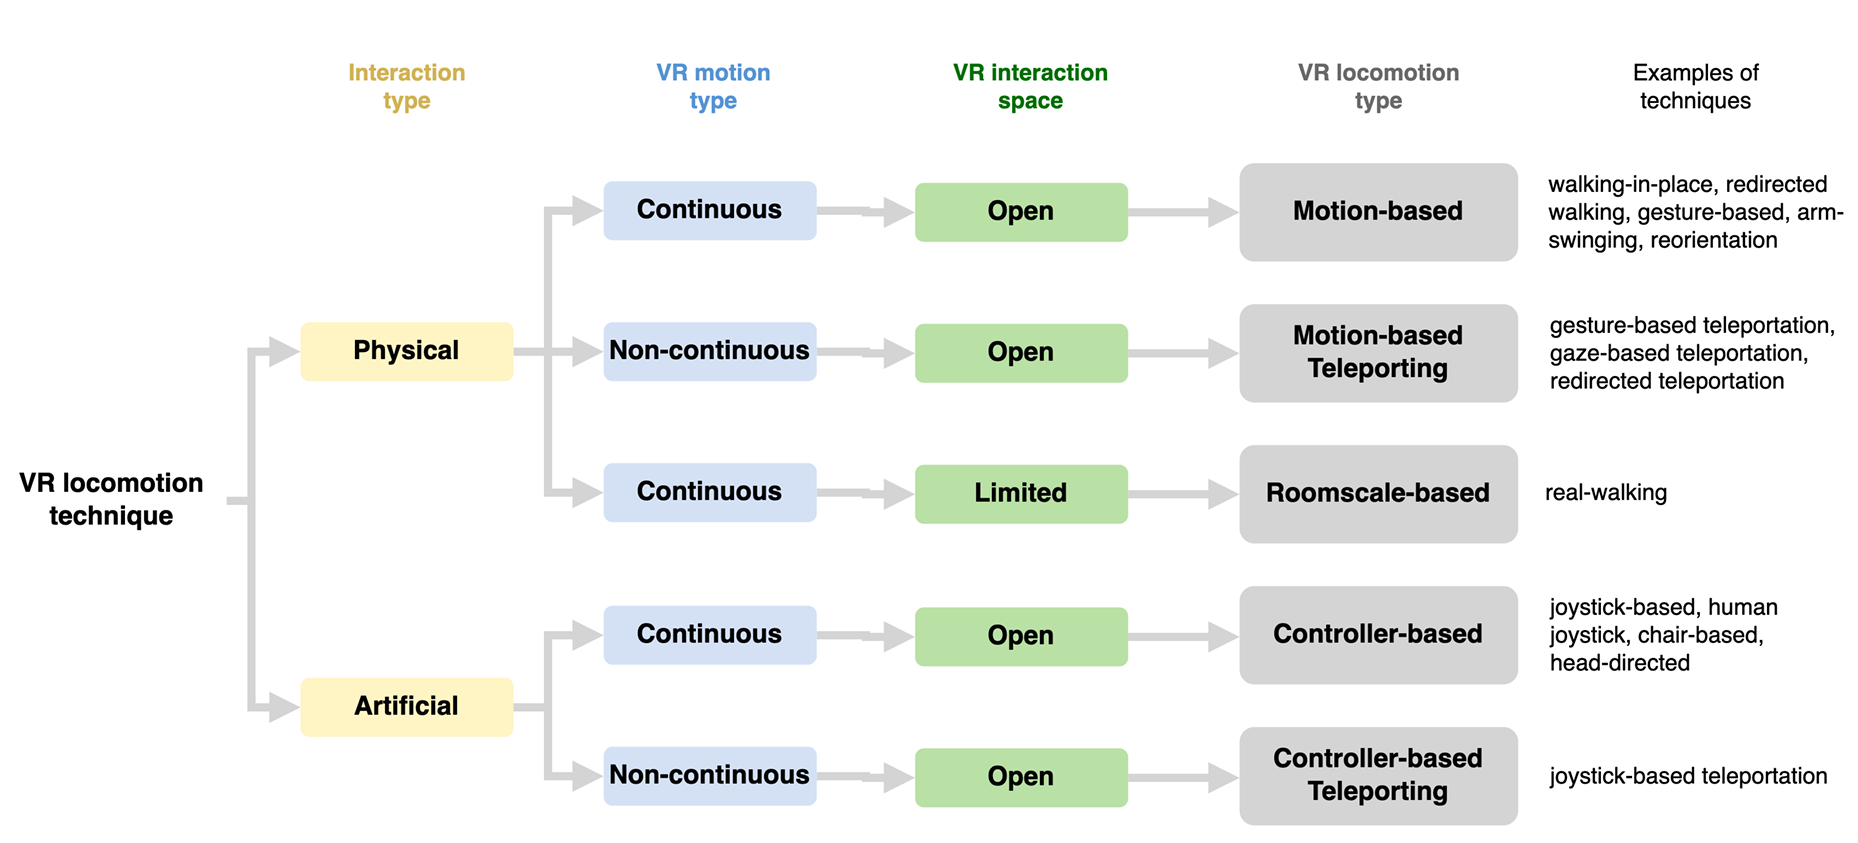
\includegraphics[width=\textwidth]{NOVAthesisFiles/Images/papers/vr-locomotion-typology.png}
    \caption{Typology of \gls{VR} locomotion techniques by Boletsis et al.\cite{Boletsis2022}}
    \label{fig:vr-locomotion-typology}
\end{figure}

Regarding the interaction type, a locomotion technique can be "physical" - 
the input is based on the user's physical movement - or "artificial" - utilizes input devices for direct \gls{VR} motion and navigation.
\gls{VR} motion types may be "continuous" - the transitions between positions is smooth and non-interrupting - 
or "non-continuous" - the transitions between positions are abrupt or instantaneous.
Finally, the \gls{VR} interaction space may be "open" - the \gls{VE} is larger the the user's physical space - 
or "limited" - the physical environment constraints the \gls{VE}'s size.

Different sets of these characteristics define the different types of 
locomotion techniques that are to be discussed in the following sections. 
It is also important to note that these techniques may be used in combination with each other, 
i.e., a technique integrating two or more other techniques \cite{Boletsis2022}.

\subsection{Joystick}
\label{sec:joystick}

Controller-Based locomotion techniques are used in an open \gls{VR} interaction space, with continuous motion and require 
an artificial means of input, such as a controller or other similar input devices\cite{Boletsis2017}.
Joystick-based locomotion is not only the most prevalent of this type of techniques, it is also one of the most used 
techniques in research \cite{Boletsis2022}.

Joystick-Based locomotion can be described in the following manner: given a user in a \gls{VE} from a \gls{VR} application, 
the way that they navigate in said \gls{VE} is dependent on a joystick controller. The joystick rests in a neutral position until the user
applies force, changing its value in a certain axis, normally from -1 to 1 (see Figure~\ref{fig:vive-joystick}). The values registered 
on the joystick's horizontal and vertical axis will make the user continuously translate from one position to the next in the 
direction related to the user's gaze direction, i.e., if the user is looking in a certain direction and applies vertical of 1 
they will move in the yaw direction of their gaze at full speed \cite{Coomer2018}.
\begin{figure}[b]
    \centering
    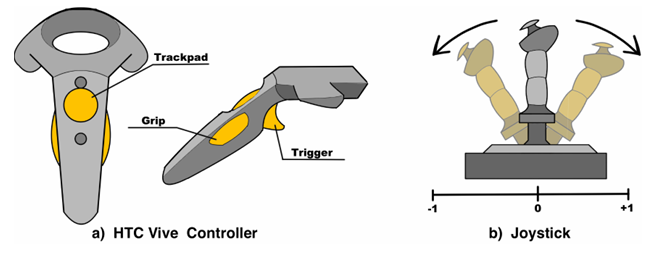
\includegraphics[width=0.75\textwidth]{NOVAthesisFiles/Images/papers/vive-joystick.png}
    \caption{Diagram of Vive Controller and Joystick \cite{Coomer2018}}
    \label{fig:vive-joystick}
\end{figure}

The artificial means of creating input for movement makes joystick locomotion considered not physically demanding and a high ease-of-use 
technique, especially noticed in users who have prior experience with similar controllers \cite{Nasiri2023}. This locomotion type also registers 
moderate-to-high levels of immersion when used, mostly due with the motion's uninterruptible nature \cite{Boletsis2019}.

Though intuitive and not physically demanding, joystick locomotion has a caveat that pertains to the user's comfort. This locomotion type can create
motion sickness, due to the conflicting movement cues from user's proprioception, their vestibular sense and from their vision, as the user 
is physically stationary whilst they move in the \gls{VE} \cite{Langbehn2018}. This is especially felt by unexperienced \gls{VR} users. \cite{Nasiri2023}

It's due to this discomfort and the lack of sufficient levels of immersion that this locomotion technique isn't the most appropriate for 
the purposes of this research, and thus it will not be implemented. [TODO: Rework this]

\subsection{Teleportation}
\label{sec:teleportation}

Teleporting differs from Controller-Based locomotion techniques in that it is non-continuous, as, 
instead of moving continuously, users are teleported from one location to the next in an interrupted manner during their navigation \cite{Boletsis2017}, 
and ,much like \nameref{sec:joystick}-Based locomotion, it is one of the most used locomotion techniques\cite{Boletsis2022}.

When teleporting, a user dictates where they want to teleport to, usually by holding down some input button on a controller and pointing to
the pertained destination with said controller, releasing said input when the destination has been chosen. On release the user 
moves to the selected destination instantaneously (see Figure~\ref{fig:teleporting}) \cite{Coomer2018, Nasiri2023}.

\begin{figure}[b]
    \centering
    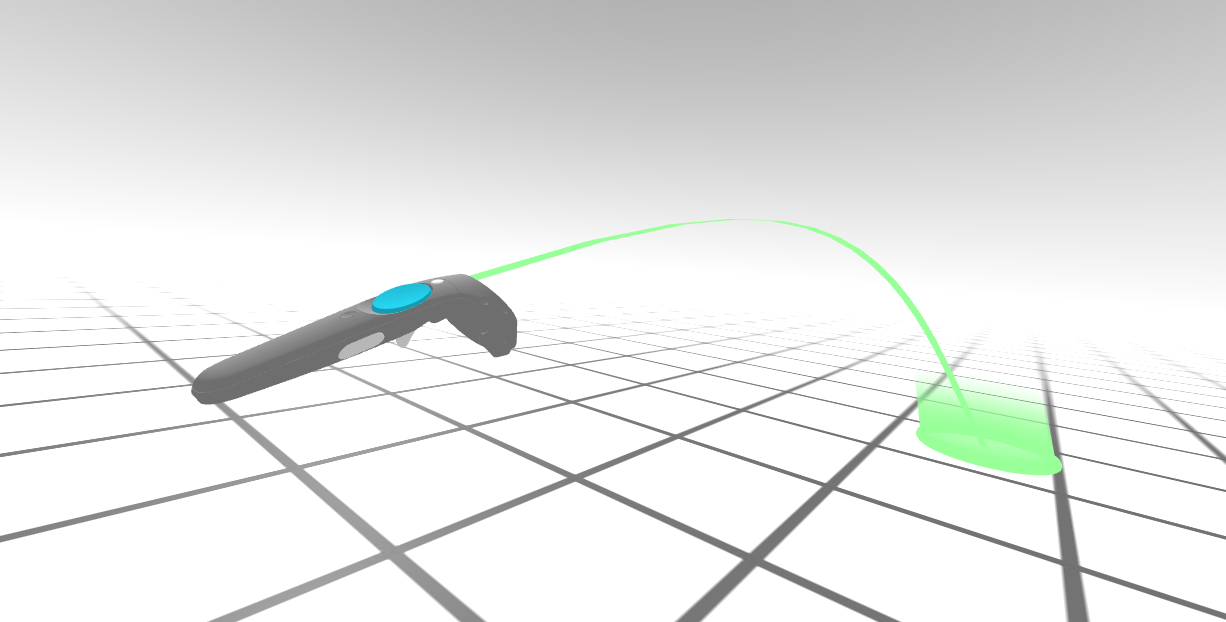
\includegraphics[width=0.6\textwidth]{NOVAthesisFiles/Images/papers/teleporting.png}
    \caption{Graphical Representation of Teleporting \cite{Coomer2018}}
    \label{fig:teleporting}
\end{figure}

The discontinuity of this locomotion methods' creates strengths and weaknesses. On the positive side, the discrete jumps prevent feelings of
cybersickness by not having a conflicting continuous motion occurring while the user is stationary \cite{Boletsis2019, Nasiri2023}, 
and is generally more efficient at covering long distances\cite{Coomer2018}. On the other hand the jumps can create some disorientation and
loss of immersion, as after teleporting the user takes more time to fully comprehend their surroundings \cite{Langbehn2018}, exerting more
cognitive effort and in turn breaking the illusion of the \gls{VE}.

To mitigate this lack of immersion, studies tried to provide less artificial manners of performing teleportation. However, even with similar or 
slightly better results in regards to immersion, users still preferred using controllers rather then the purposed controller-free \cite{Bozgeyikli2016}, 
and even hands-free teleportation techniques \cite{Prithul2022}.

Even so, in various comparison studies, teleportation has been identified as a preferred locomotion method over other frequently used 
alternatives, mostly due to the lack of motion sickness and high ease-of-use \cite{Boletsis2019, Langbehn2018}.

Although comprehending this technique's strengths and weaknesses is important for the full understanding of the problem at hand, teleporting proves 
to be a non suitable technique for this research, due to the lack of immersion it provides, and therefore its implementation was not considered.

\subsection{Omni-Directional Treadmills}
\label{sec:omni-directional-treadmills}

As a type of locomotion techniques that require physical interaction for continuous motion in open \gls{VR} interaction spaces, 
Motion-Based techniques are rooted on the user's physical movement for their navigation in a \gls{VE} \cite{Boletsis2017}, which poses the
question: How can a user physically navigate a \gls{VE} larger than their physical environment without reaching the limits 
of their available space?

According to Nilsson et al. \cite{Nilsson2018}, it's possible to identify yet another three sub-types of Motion-Based 
locomotion techniques, all of which try to solve this problem, with these being Repositioning Systems, Proxy Gestures and 
Redirected Walking.

Repositioning Systems refer to input devices that try to counter-act users' forward motion when walking, essentially keeping them in place, 
ranging from more devices with a more "active" approach to the repositioning like treadmills to more "passive" options like friction-free
platforms Figure~\ref{fig:repo-systems}.

\begin{figure}[b]
    \centering
    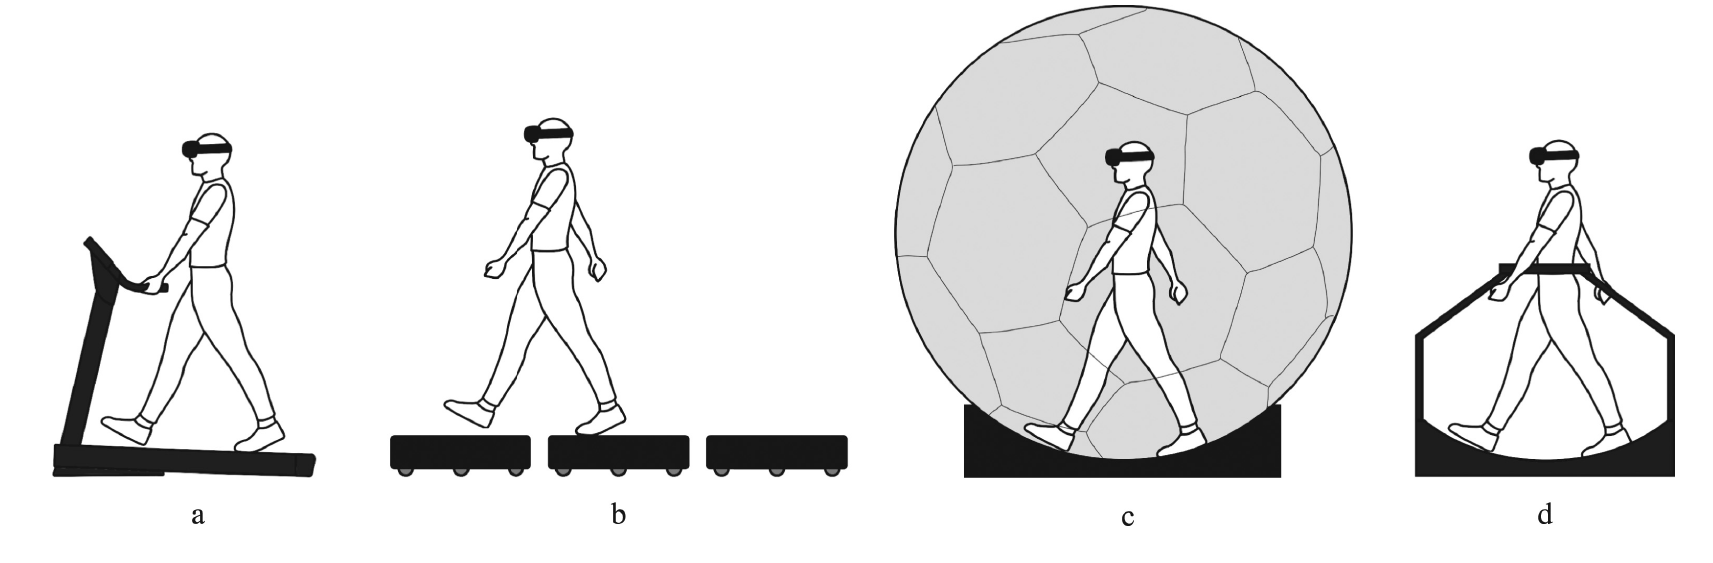
\includegraphics[width=\textwidth]{NOVAthesisFiles/Images/papers/repo-systems.png}
    \caption{Four examples of repositional systems: (a) Traditional Linear Treadmill, (b) motorized floor tiles,
    (c) a human-sized hamster ball, and (d) a friction-free platform. \cite{Nilsson2018}}
    \label{fig:repo-systems}
\end{figure}


One of the most common Repositioning Systems are Omni-Directional Treadmills - devices that sense the direction of users' steps whilst 
walking in a 360 degree space, maintaining the user at the center of their available space, translating the users steps as movement in the \gls{VE}.
User studies seem to indicate that the motion caused, although not reaching quite exactly the feeling of real walking (with some users indicating a 
feeling more similar to running or skating rather than walking), this locomotion method evokes high levels of presence, similar to real walking \cite{Syamil2024}.

However, despite taking an almost accurate walking motion as input, offering high levels of immersion and providing a promising solution 
for the physical limitations of walking in a constricted space, these devices are often expensive and tend to be difficult to operate \cite{Cherni2020}.
In addition, performing quick turns or side-steps may cause users to lose balance \cite{Nilsson2018} and more natural walking techniques 
like the later discussed \nameref{sec:redirected-walking} are preferred by users \cite{Syamil2024}. It's for these reasons that this research 
pretends to provide a more suitable, immersive and affordable alternative to a technique like Omni-Directional Treadmills, thus this technique
was not chosen for further study and/or improvement in this research.  


\subsection{Walking-In-Place and Arm-Swinging}
\label{sec:wip-and-as}

Proxy Gestures techniques, contrarily to Repositioning Systems like the \nameref{sec:omni-directional-treadmills}, offer inexpensive 
and easy-to-learn solutions to the problem caused by physical constraints during Motion-Based locomotion techniques \cite{Nilsson2018}. 
Locomotion in these techniques is based on gestures that emulate walking motions, keeping users moving their limbs, but 
stationary at the same time.

Walking-In-Place is the most common of these techniques \cite{Boletsis2019,Nilsson2018}. To emulate walking, users perform a 
gesture comparable to "marching on the spot" in order to move in the direction they are facing, sometimes relying on sensors for 
detecting the legs' movements \cite{Cherni2020}, yet the detection can recur solely to \glspl{HMD} \cite{Lee2018}.

Although it might sound counter-intuitive for simulating physical walking, Arm-Swinging is a technique that switches the 
motion performed by users from the lower body to the upper body. In this technique users swing their arms back and forth interchangeably, 
to move in the direction they are facing. The objective is to perform a gesture comparable to how humans naturally swing their 
arms when they walk, with the arm's movements being detected either by armband-like sensors \cite{Cherni2020}, or just by 
controllers users hold in their hands \cite{Coomer2018}.

The fact that both these techniques have the capability to only rely on \glspl{HMD} and their associated 
Controllers makes them more accessible, easier to use and thus a more prevalent technique 
for common users \cite{Nilsson2018}. Additionally, the motion-based input provides a more appropriate proprioceptive feedback 
similar to real walking than \nameref{sec:joystick} and \nameref{sec:teleportation} 
techniques and hence usually grade higher in immersion ratings \cite{Boletsis2019}. 

Despite this, these techniques present some caveats. Walking-In-Place can be physically demanding and potentially 
induces motion sickness after prolonged use \cite{Boletsis2019,Cherni2020}, making it not the best solution for use-cases 
in which users have to navigate an extensive \gls{VE}. Arm-Swinging, although not in the same magnitude, is also limited by this 
weak point \cite{Coomer2018}, but it is additionally limited by the fact that users can't use their arms for interaction 
while moving \cite{Nilsson2018}. 

Although both techniques prove useful for addressing the problems caused by physical limitations while moving, 
their strong points and weak points indicate them as non suitable for the context of this research. [TODO: Rework this]


\subsection{Redirected Walking}
\label{sec:redirected-walking}

Motion during navigation in \gls{VR} is an added value to immersion. The previously mentioned techniques - \nameref{sec:omni-directional-treadmills},  
\nameref{sec:wip-and-as} - proved this, since they are regarded as high immersion techniques compared to techniques with artificial means of 
input (\nameref{sec:joystick} and \nameref{sec:teleportation}), due to their reliance on gestures that simulate walking \cite{Nasiri2023}.
Additionally, Motion-Based techniques also tend to score higher in spatial orientation/awareness, compared to artificial means \cite{Cherni2020,Coomer2018}.
Even so, users tend to prefer using \gls{RDW} over these techniques \cite{Langbehn2018, Syamil2024}.

\gls{RDW} is not a particular technique, but rather an umbrella term for all techniques that allow users to physically walk in a 
\gls{VE} by controlling their path in ways that keep them from reaching the edges of their available physical space \cite{Nilsson2018}. 
Despite the multitude of possible implementations, \gls{RDW} aims to follow 4 criteria: \textbf{Imperceptibility} - users should be as less aware 
as possible of the redirection taking place - \textbf{Safety} - users should feel as safe as possible from reaching the boundaries of their 
available physical space - \textbf{Generality} - the technique's correct functionality should be as independent as possible from the physical 
environments in which they might be used - and \textbf{Absence of Unwanted Side-Effects} - the technique should aim to be devoid of 
side-effects as those of cybersickness and disorientation \cite{8255772}.

Literature on this topic has recognized two common types of redirection strategies adopted by these techniques \cite{8255772, Nilsson2018}:
\begin{itemize}
    \item \textbf{Perspective Manipulation} - 
    RDW techniques that steer users away from the edges of their tracking space by manipulating the mapping between the user's real 
    and virtual movements. Manipulation is accomplished by applying repositioning and orientational transformations, like gains to 
    the users translational and rotational movements
    i.e. if a gain of 2.0 is applied to the user's 
    forward translation, then they will travel twice as fast in that forward motion in the \gls{VE}
    
    \item \textbf{Environment Manipulation} - 
    These techniques rely on the \gls{VE}'s layout and characteristics in order to accomplish redirection. This is done by either 
    building a \gls{VE} with a pretended path or by changing the \gls{VE}'s properties whilst the user is navigating it, in order to change 
    the users' routes and keep them away from the limits of their available space.
\end{itemize}

To further categorize these techniques, Suma et al.\cite{6180877} purpose a taxonomy of techniques (observable in Figure~\ref{fig:rdw-taxonomy}) 
according to whether these 
are \textbf{Repositioning Techniques} - techniques that compress the \gls{VE} by manipulating the correspondence between points in the real 
and virtual environments - and \textbf{Reorientation Techniques} - techniques that attempt to rotate the user's facing direction away from 
the edges of their tracking space. These techniques can then be \textbf{Overt} - easily noticed by users - or \textbf{Subtle} - changes are 
hidden from users - and either \textbf{Continuous} - the changes are slowly applied - or \textbf{Discrete} - changes are immediate.
\begin{figure}[t]
    \centering
    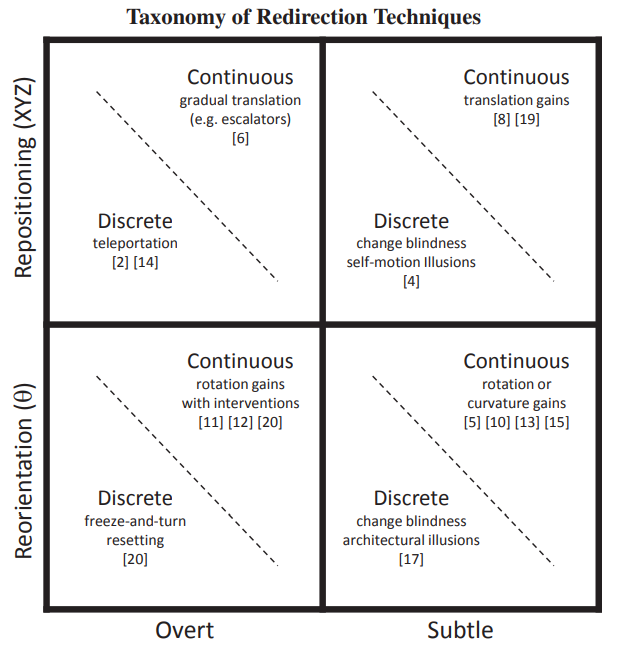
\includegraphics[width=0.55\textwidth]{NOVAthesisFiles/Images/papers/rdw-taxonomy.png}
    \caption{ Taxonomy of redirection techniques for supporting natural
    walking through immersive \glspl{VE}. The vertical axis
    distinguishes how the technique is applied in the environment. The
    horizontal axis provides a ranking in terms of notability to the user.
    The division in cells represents distinct implementation strategies for
    each type of technique. \cite{6180877}}
    \label{fig:rdw-taxonomy}
\end{figure}

\textbf{Subtle Continuous Repositioning} and \textbf{Reorientation} techniques are associated with the use of Translational and 
Rotational Gains, respectively, and these could be considered the most prevalent techniques of the mentioned 
Perspective Manipulation strategy for redirection \cite{Nilsson2018}. These gains compress the \gls{VE} by deliberately altering the 
mapping between the users' movements in the physical and virtual spaces (Figure~\ref{fig:rdw-gains}). 
Translation Gains scale the users' steps, whilst Curvature 
Gains are a continuous small rotations applied while the user is walking forwards, creating the possibility for users to walk infinitely 
along a virtual path while walking in circles in their tracking space. Bending Gains are another type of gain that works similarly to 
Curvature Gains, but these are used in already curved virtual paths. Both Curvature and Bending Gains require either \textit{a priori} 
knowledge or a good prediction method of the path users take in the \gls{VE} \cite{8255772}.

Most of the techniques in this taxonomy are associated with a Perspective Manipulation strategy. However, 
\textbf{Subtle Discrete Reorientation} techniques do directly alter the \gls{VE} making them accurately follow the
Environment Manipulation strategy. Change blindness redirection \cite{5759455} serves as an example of how a technique 
like this might be used, as it discreetly makes changes to the environment outside users' \gls{FOV}, leading them to take different 
paths without breaking immersion.

With the given nomenclature, \textbf{Subtle Discrete Repositioning} might seem counter-intuitive, for how can a \gls{VR} application 
make discrete jumps in users' positions without their awareness? Bruder et al. \cite{Bruder2011} purposed a solution by creating visual 
optic flow effects, reminiscent of filters or tunnel vision, to mask the discrete jumps in the users position. User studies performed 
with the implementation of this technique revealed that users weren't able to discern the difference between real and virtual movements 
while influenced by the technique, proving that this it succeeds in its imperceptibility.

\begin{figure}[t]
    \centering
    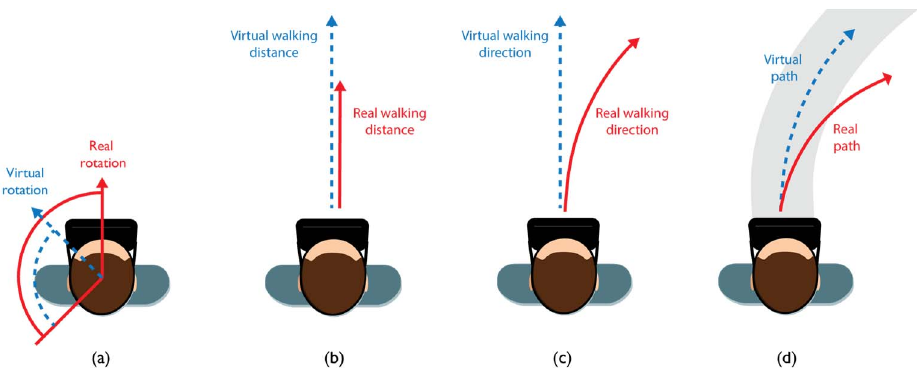
\includegraphics[width=0.75\textwidth]{NOVAthesisFiles/Images/papers/rdw-gains.png}
    \caption{  Illustration of four types of gains used to manipulate the mapping between the user’s real
    and virtual movement: (a) rotation gains (user stationary), (b) translation gains (user moving
    forward), (c) curvature gains (user moving forward), and (d) bending gains (user moving on a
    curve). \cite{8255772}}
    \label{fig:rdw-gains}
\end{figure}

As mentioned, \gls{RDW} techniques should aim to be as unnoticeable as possible \cite{8255772}, but overt techniques prove valuable in 
limiting conditions to assert that the technique is safe for use. \textbf{Overt Discrete Reorientation} techniques are associated with 
techniques used to redirect users to the available space when they are near of its limits. Freeze-and-turn is an exemplary 
"failsafe" emergency technique \cite{Williams2007} . When a user is nearing the edge of 
their tracking space, the display on the users' \glspl{HMD} freezes and prompts them that 
a reset is required. Once the user has completed a 180 
degree turn, the display resumes. Even if the redirection is easily noticeable, Safety can be prioritized over 
Imperceptibility for extreme cases such as these.

\textbf{Overt Continuous Reorientation} techniques are then comparable to the previously mentioned type of technique. The difference lies 
in the fact that when the system is resetting, the display doesn't freeze, as when the user is prompted to turn 180 degrees, they're movements 
are being translated as a full 360 degree turn in the \gls{VE}, allowing them to proceed their virtual path without reaching the edges of 
their tracking space.

\textbf{Overt Discrete Repositioning} relies simply on teleporting the user from one position to the next, which may be disorienting if 
users aren't given enough context and aren't expecting the instantaneous change in space. This is mitigated through the use of portals, 
making the transition more deliberate and potentially a more immersive experience \cite{6180877}. This serves as an example that 
overt techniques don't necessarily reduce feelings of presence in a \gls{VE}. 

\textbf{Overt Continuous Repositioning} techniques simply translate the virtual environment about the user's position continuously, in order 
to achieve repositioning. This then allows the user to walk on areas in the virtual environment that were not previously
accessible within the confines of the physical workspace. To minimize the jarring sensations these techniques may feel, they can be coupled 
with the use of known metaphors associated with motion such as escalators, elevators and vehicles.

It's important to note that techniques may incorporate more than one of the mentioned strategies and types of techniques. The work by 
Rebelo et al. \cite{Rebelo2024} is an example of this, as the developed techniques rely on the use of portals, alteration of the \gls{VE}'s 
structure and translation gains, in order to permit the navigation of an extensive \gls{VE} in a room-scale physical space.

It is also relevant to note that \gls{RDW} techniques present caveats. These techniques typically need larger physical environments in order to be 
imperceptible \cite{Langbehn2018}, since smaller tracking spaces imply the need for higher value gains and gains need to stay below detection 
thresholds to remain imperceptible, and thus immersive \cite{Grechkin2016}. Minimum room sizes and the mentioned gain thresholds are dependent on 
the techniques being used and remains a challenge for \gls{RDW} research. 

Techniques like Telewalk \cite{Rietzler2020} directly address this limitation, 
as this technique aims to be a locomotion approach that permits navigation in VR in a more natural way to increase presence and immersion, in 
spaces as small as 3x3 meters. It relies on using intentionally overt Rotational and Translational Gains, with the addition of head-based direction 
control and visual indicators to help redirect users into an optimal path, as seen in Figure~\ref{fig:rdw-telewalk}. The user study conducted 
by Rietzler et al. \cite{Rietzler2020} compared Telewalk with \nameref{sec:teleportation}, since, as mentioned previously, the latter is also highly 
optimal for use-cases in which the tracking space is reduced. Telewalk did result in stronger feelings of presence and immersion and was 
seen as more natural than Teleportation, mostly accomplishing its purpose, yet users were evenly divided in terms of preference between the two 
techniques. This was mostly due to an unwanted side effect created by the overtness of the technique, which leads to the next limitation of 
\gls{RDW}.

\begin{figure}[b]
    \centering
    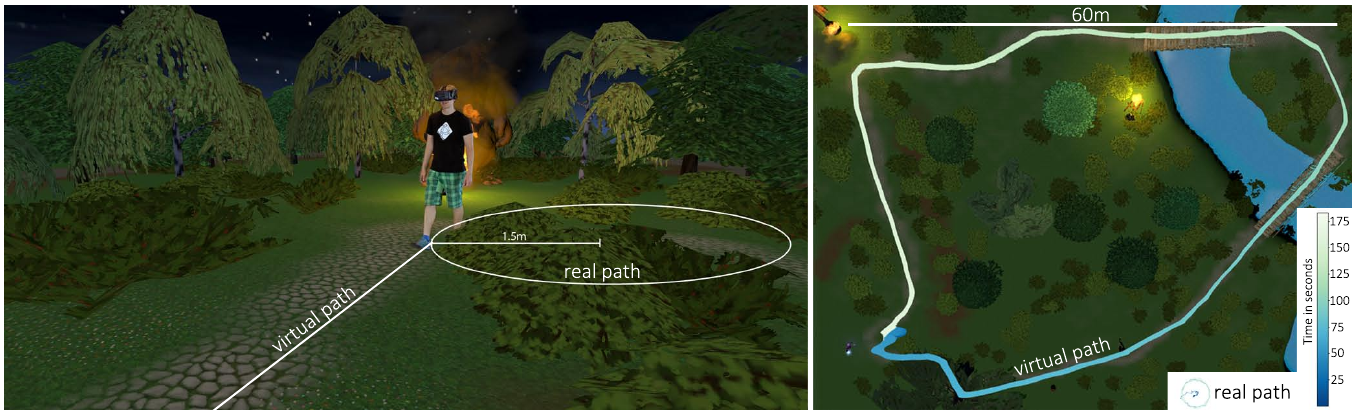
\includegraphics[width=\textwidth]{NOVAthesisFiles/Images/papers/rdw-telewalk.png}
    \caption{The concept of Telewalk: The combination of perceivable curvature and translation gains along with a head based camera
    control allows to compress any virtual space to a pre-defined real world radius (in our case 1.5m). (Left) illustration of walking paths
    and (right) plots of the virtual and real path walked in our study application. \cite{Rietzler2020}}
    \label{fig:rdw-telewalk}
\end{figure}

\gls{RDW} techniques that create a large mismatch between real and perceived motion by using high translational gains 
can cause \gls{VR} sickness \cite{Gemert2024}, as well as an increased cognitive load, particularly when overt redirection techniques 
are applied \cite{8255772}. The effects vary depending on user characteristics, hardware, and gain configurations, thus 
an exact relationship between \gls{VR} sickness and \gls{RDW} remains unclear and a challenge in \gls{VR} research \cite{Gemert2024, Grechkin2016}.

This is one of the challenges to be tackled in this research. After exploring the literature of Locomotion techniques, 
it is safe to say that \gls{RDW} techniques provide better levels of immersion and presence in the navigation of a \gls{VE}. It is, however, 
limited by the mentioned weak points, but, due to the diverse possibilities of implementations these type of locomotion technique allows, 
alternatives that mitigate the problems created by these limitations can still be explored and refined. Thus, the accomplishing of this 
research's objectives involve the use of the mentioned strategies and techniques of \gls{RDW}.


%\subsection{Summary}
%\label{sec:loc-summary}

%[TODO: Present table with techniques, comparing strong and weak points]

%[TODO: Go over why continuous motion-based locomotion provided by RDW is the most relevant for this research 
%and connect it with the Motivation (address the gap for high immersion yet physically limited locomotion)]

\section{Non-Euclidean Spaces in VR}
\label{sec:non-euclidean-space}

As discussed in the \nameref{sec:navigation-in-ves} section, literature seems to agree that Navigation employs mental effort, mainly through the 
act of intaking and keeping of spatial information, which is supported by the use of the denominated cognitive/mental maps \cite{Eastgate2014}. 
Being a mental representation of spatial data, its understanding is quite limited, although it is arguably instinctive to call it a 
"picture in our heads", yet studies as those of William Warren \cite{Warren2019} reveal that this is inaccurate.

Warren's experimental biology study \cite{Warren2019} defies Navigation assumptions, by exploring Non-Euclidean spaces in \gls{VR}. 
Our perception of the real world is bound to the rules of 3 Dimensional Euclidean Geometry, and thus Non-Euclidean Spaces refer to spaces 
in which these rules are altered or do not apply, being then bound to a Non-Euclidean Geometry . This section's purpose is to explore 
two varieties of Non-Euclidean Spaces and their use in \gls{VR}: \nameref{sec:impossible-spaces}, which modify the geometric rules of distance, 
and \nameref{sec:hyperbolic-spaces}, which alter the Euclidean's classic Parallel Postulate - given a line and a point not on that line, 
only one parallel line can be drawn through the point \cite{Pisani2019}.

If one was to store spatial knowledge onto an Euclidean mental map, it would be conclusive that traversing a Non-Euclidean Space would prove to be 
disorienting, yet Warren's study proves the contrary \cite{Warren2019}. In this \gls{VR} experiment, two groups of users had to traverse a maze, yet one group traversed the maze normally
whilst the other traversed a maze with the inclusion of invisible wormholes that seamlessly transported them from one position to another creating
a Non-Euclidean Impossible space, as seen in Figure~\ref{fig:warrens-mazes}. The mazes contained objects and the two tasks of the study  
consisted on firstly finding the objects and the routes between them, and then participants were asked to go one object to another in the shortest 
route possible without the mazes' structures, 
relying only on their spatial knowledge. The results on Figures \ref{fig:warrens-mazes} and \ref{fig:warrens-mazes-paths} show that 
the participants of the Non-Euclidean maze revealed a clear bias towards the use of the wormholes. Warren states that these results are in agreement 
with his hypothesis that spatial knowledge is represented as Cognitive Graphs, rather than Cognitive Maps, since despite the the irregularities 
caused by the wormholes, participants consistently relied on local metric cues and graph-like relational behavior. 

With Warren's demonstration, it's conclusive that Non-Euclidean Spaces are primed for \gls{VR} use. In the next sections, the advantages that this 
type of spaces have for \gls{RDW} will be explored.


\begin{figure}[p]
    \centering
    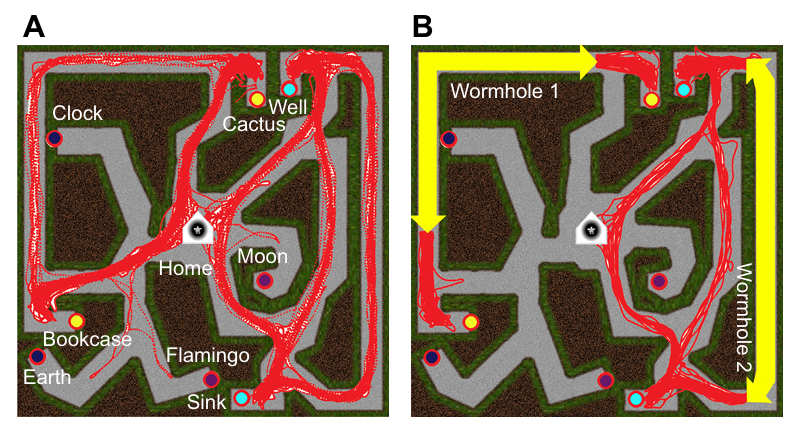
\includegraphics[width=0.75\textwidth]{NOVAthesisFiles/Images/papers/warrens-mazes.png}
    \caption{Traversed mazes in Warrens' study, where A is the "normal" Euclidean maze, whilst B is the Non-Euclidean maze with Wormholes that seamlessly
    translate a user from one location to the next. Red lines indicate the paths users took.  \cite{Warren2019}}
    \label{fig:warrens-mazes}
\end{figure}

\begin{figure}[p]
    \centering
    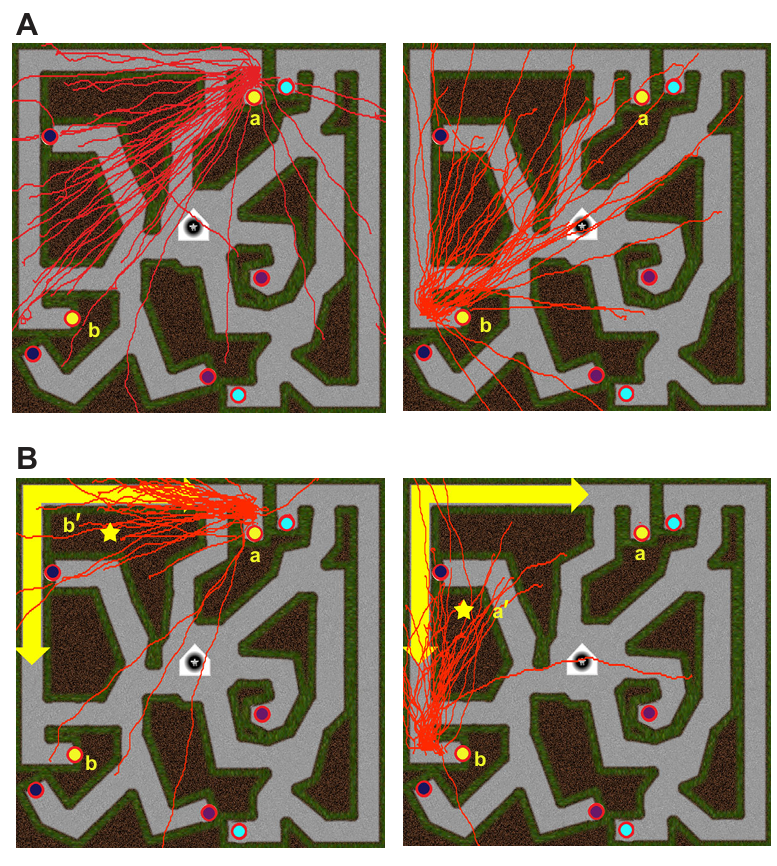
\includegraphics[width=0.75\textwidth]{NOVAthesisFiles/Images/papers/warrens-mazes-paths.png}
    \caption{Paths taken between objects Bookcase and Cactus in Euclidean maze A and Non-Euclidean maze B. 
    Stars in maze B indicate the location of the object in Non-Euclidean coordinates. The dense amount of paths in the direction of these 
    stars show that participants' Wayfinding was highly biased by the Wormholes. \cite{Warren2019}}
    \label{fig:warrens-mazes-paths}
\end{figure}


\subsection{Impossible Spaces}
\label{sec:impossible-spaces}

Fictional works like BBC's science-fiction TV show \textit{Doctor Who} include spaces that defy the physical laws of our reality, 
such as the TARDIS, the iconic spaceship that is "bigger on the inside", to increase the sense of wonder in their narratives. 
It was not long after the "second-wave of \gls{VR} development" \cite{Anthes2016} that fans of the show tried to recreate this feeling of 
wonderment by bringing the famous police box to life through the use of \gls{VR}, due to its immersive capabilities
\footnote{TARDIS VR by itch.io user \textit{feroxxy} - \href{https://feroxxy.itch.io/tardisvr}{https://feroxxy.itch.io/tardisvr} - Last Access: Jan 2025 } 
. This project and the previously mentioned study by Warren \cite{Warren2019} are prime examples of what Impossible Spaces are and their 
general application in \gls{VR}

\begin{figure}[b]
    \centering
    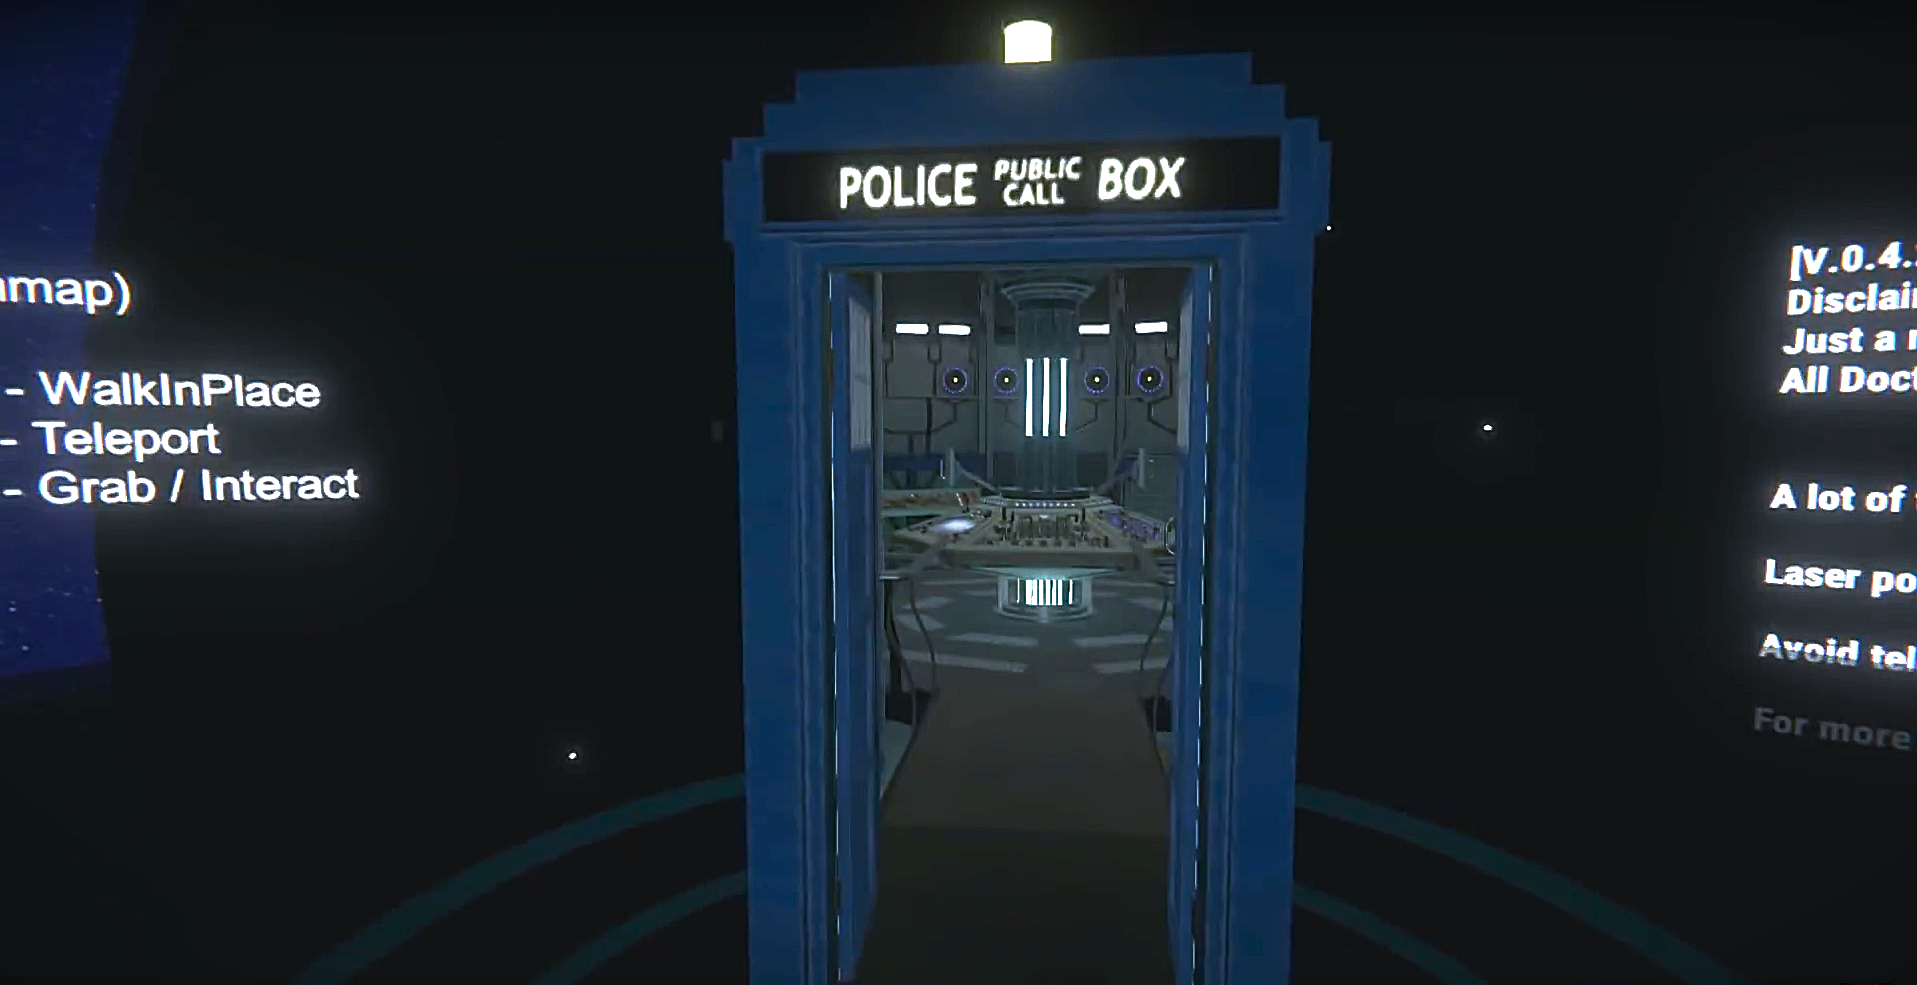
\includegraphics[width=0.85\textwidth]{NOVAthesisFiles/Images/papers/tardis.png}
    \caption{A screenshot of the TARDIS VR project, depicting the famous police box that is "bigger on the inside", one of the possible ways to 
    depict an Impossible Space in \gls{VR}.}
    \label{fig:tardis}
\end{figure}

Impossible Spaces are, in the majority of cases \cite{Lochner2021}, experiences taking place in \glspl{VE} that violate the rules of Euclidean 
Space, yet keep the appearance of the real world by keeping most of its Euclidean Geometry intact. This creates large \glspl{VE} that are essentially 
multiple Euclidean spaces that look ordinary when experienced locally, but when their topology is inspected, it's clear that
these spaces are connected in a matter that is physically impossible. This creates the often called "Self-Overlapping Architectures" \cite{Lochner2021, Suma2012}.

These \glspl{VE} capitalize on the lack of physical restrictions to create an architecture that fits within users' physical spaces,
granting them the ability to naturally walk in a much larger \gls{VE} by
redirecting them away from the edges of their tracking space \cite{Fisher2017, Suma2012, 6550194}, 
hence its use is considered a form of \gls{RDW} \cite{8255772}.
Given that \gls{RDW} is one of the highest immersive methods of locomotion, due to the walking motion it employs, 
as seen in the previous \nameref{sec:redirected-walking} section, 
in conjunction with the fact that users perceive the local environment as an Euclidean space, since distance 
perception is accurate by norm \cite{Barwulor2020}, Impossible Spaces provide a highly immersive \gls{VR} experience. 

The illusion of the self-overlapping architecture is mostly unnoticeable, especially when users are naive to the manipulation at hand 
\cite{Suma2012}. Distractors, visual and auditory feedback, and contextual environmental events are potential auxiliary methods to 
raise the \gls{VE}'s level of immersion \cite{Ciumedean2020,Fisher2017}, since these methods help lower the overtness of the redirection that is 
taking place.

\gls{VR} applications typically use two main methods to connect the various sections of a Self-Overlapping Architecture: 

\begin{itemize}

    \item \textbf{Transitioning Areas} - Transitional spaces that link different sections by recurring to the previously discussed 
    "change blindness" redirection technique. These areas are usually curved corridors that restrict users' \gls{FOV}, 
    allowing for the mentioned changes to happen without the users knowledge \cite{5759455, Vasylevska2017} (Figure~\ref{fig:transioning-areas}).
    
    \item \textbf{Portals} - As discussed in the \nameref{sec:redirected-walking} section, 
    the instantaneous teleportation caused by Overt Discrete Repositioning \gls{RDW} techniques could be highly disorienting if the user is 
    not prepared or doesn't have the context for such repositioning. Portals help mitigate the overtness of this technique, serving as preview 
    to the location the user is going to teleport to after passing through it \cite{Freitag2014,Lee2018}. The transition between the locations can 
    be seamless, like the wormholes from the previously mentioned study by William Warren \cite{Warren2019}, 
    making the teleportation even less noticeable, and therefore, more immersive. 
    The "Non-Euclidean Worlds Engine" project 
    \footnote{Video on the "Non-Euclidean Worlds Engine" by \textit{Code Parade} - \href{https://youtu.be/kEB11PQ9Eo8}{https://youtu.be/kEB11PQ9Eo8} - Last Access: Jan 2025 }
    provides several examples in which these portals might be used (Figure~\ref{fig:self-Overlapping}).

\end{itemize}

\begin{figure}[b]
    \centering
    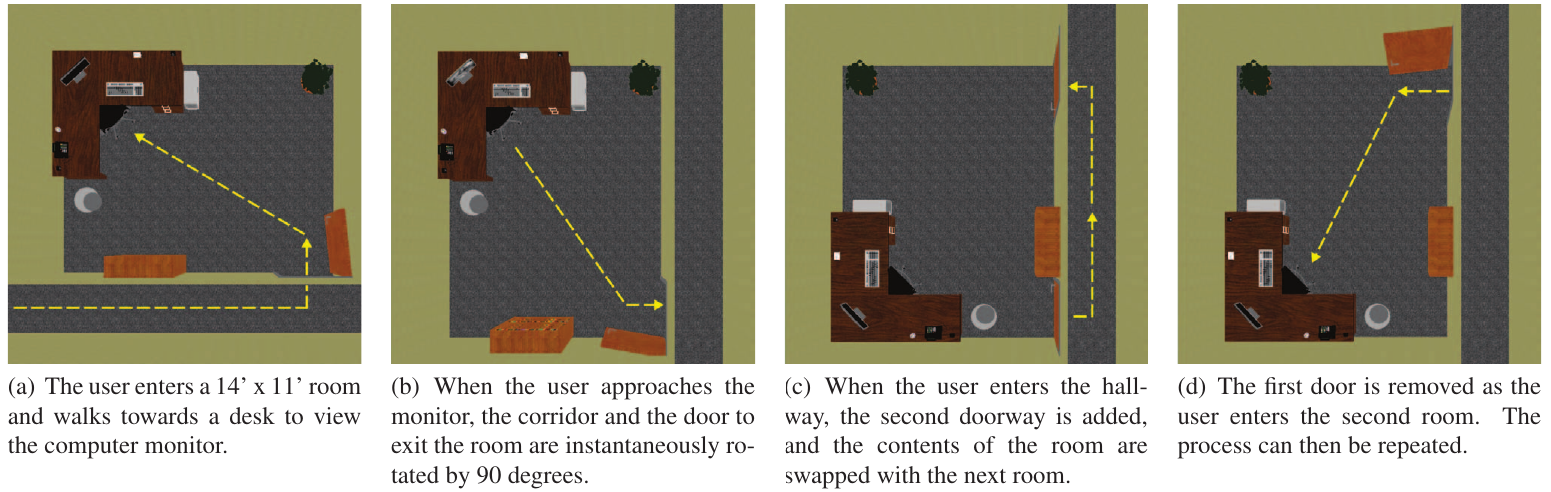
\includegraphics[width=\textwidth]{NOVAthesisFiles/Images/papers/transioning-areas.png}
    \caption{A step-by-step explanation of a possible implementation of change blindness redirection through the use of a Transitioning Area. 
    \cite{5759455}}
    \label{fig:transioning-areas}
\end{figure}

\begin{figure}[t]
   \centering
    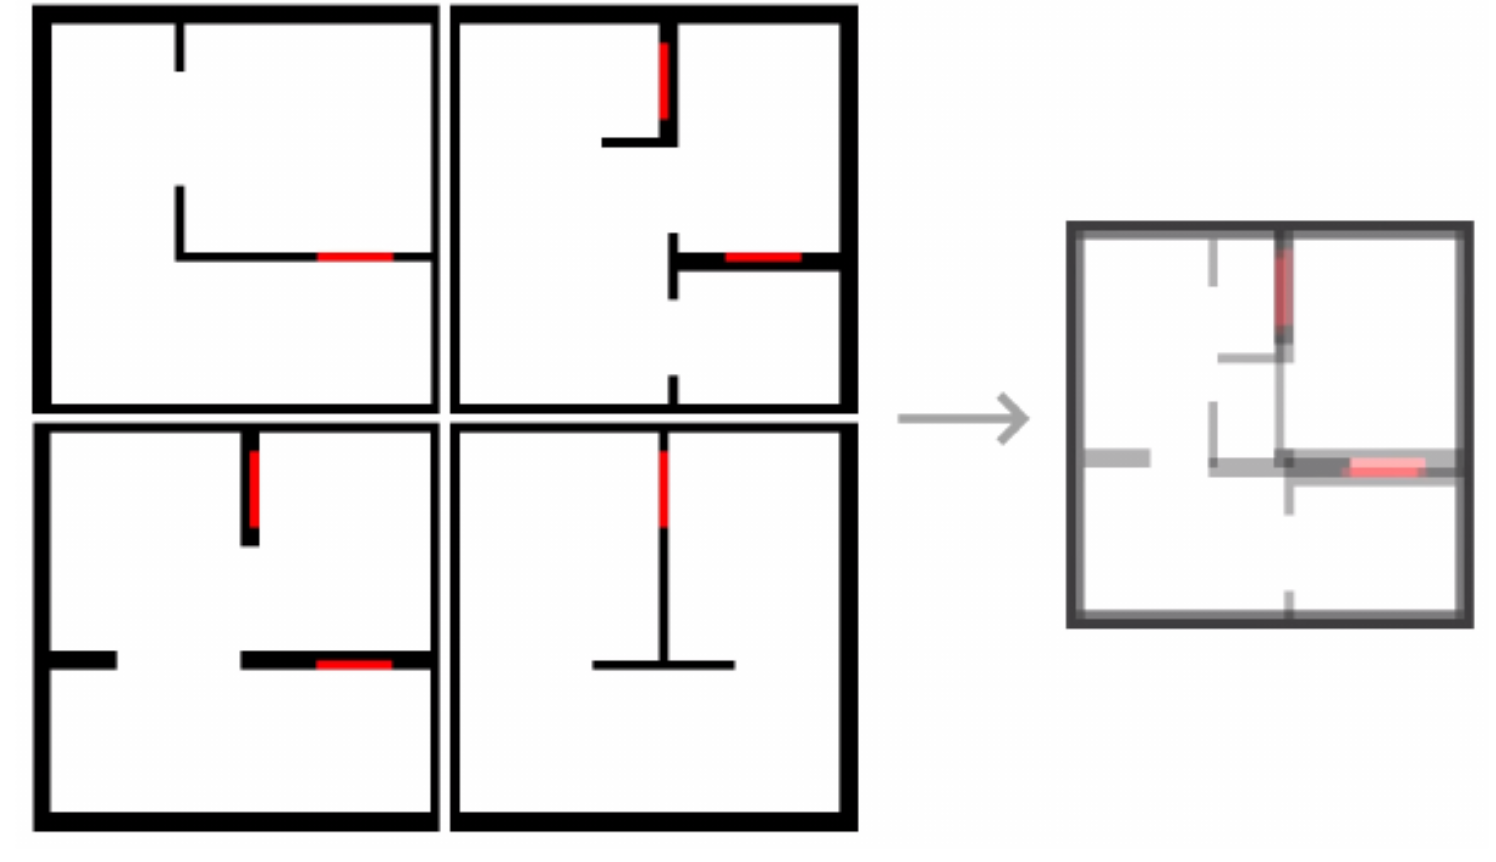
\includegraphics[width=0.5\textwidth]{NOVAthesisFiles/Images/papers/self-overlapping.png}
    \caption{A visual representation of a self-overlapping architecture from the "Non-Euclidean Worlds Engine" project.
    The four separate rooms (left) are merged together (right) through the use of portals represented in red, compressing them into a 
    \gls{VE} that only requires a physical space four times smaller than the one occupied by the four rooms.}
   \label{fig:self-Overlapping}
\end{figure}

The use of Impossible Spaces proves to be an optimal solution to map a large \gls{VE} into a limited physical tracking space, and it's applications 
with \gls{RDW} techniques seem to be extensive, all depending on the context and needs the \gls{VR} application is being developed.
Flexible Spaces, developed by Vasylevska et al. \cite{6550194}, serves as an example of how extensive these possibilities can be,
as it is a combination of the mentioned techniques, that in conjunction with the later addressed \nameref{sec:pcg}, 
creates an all-in-one dynamically adjustable redirection technique. 

\subsection{Hyperbolic Spaces}
\label{sec:hyperbolic-spaces}

As stated before, Non-Euclidean Geometry is a variant of Euclidean Geometry, by having its axioms changed, one of them 
being Euclid's Parallel Postulate.
It states that through any given point not on a line there passes exactly one line parallel to that line in the same plane\cite{Eryk2018}. 
If one were to change this axiom to either permitting the existence of two or more parallel lines or restricting it to no parallel lines, 
they would get Hyperbolic and Elliptic Spaces, respectively \cite{Pisani2019}.


Hyperbolic Spaces are then infinite by definition, having more space available in a given distance than in Euclidean Spaces, presenting a 
constant negative curvature \cite{Pisani2019}. Its properties make it valuable for the representation of relational data, as its infinity allows 
integrate trees of data with deliberately large sizes, proving more useful than Euclidean Graphs \cite{Eryk2017, Liu2019}. 
An example of this is the hyperbolic graph of GitHub's most used languages,created by Celiska et al. \cite{Celiska2017} and represented in 
Figure~\ref{fig:github}, 
in which the distances between the languages' nodes indicated how frequently these were used together.

\begin{figure}[t]
    \centering
     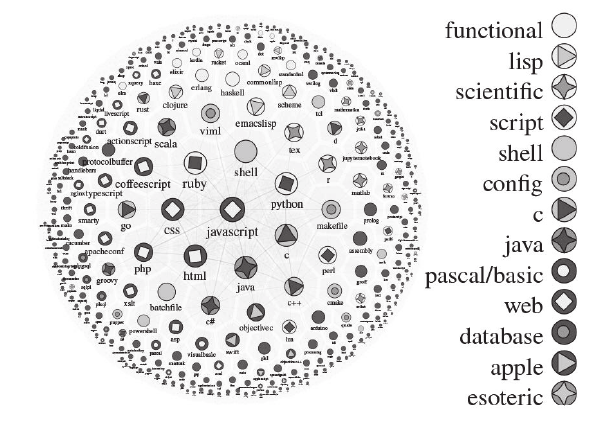
\includegraphics[width=0.6\textwidth]{NOVAthesisFiles/Images/papers/github.png}
     \caption{Hyperbolic graph of GitHub's most used languages. The closer the languages' nodes are, the more frequently these 
     languages are used together.\cite{Celiska2017}}
    \label{fig:github}
 \end{figure}

Entertainment has also benefited from Hyperbolic Geometry in the video-game industry, as games like \textit{Hyperbolica} (Figure~\ref{fig:hyperbolica})
\footnote{Hyperbolica Steam page - \href{https://store.steampowered.com/app/1256230/Hyperbolica/}{https://store.steampowered.com/app/1256230/Hyperbolica/}, Last Access - Jan 2025 } 
and \textit{HyperRogue} \cite{Eryk2017}
have integrated hyperbolic spaces into their gameplay to create challenging puzzles and situations for players to solve. 
With the seamless integration of Hyperbolic Spaces in video games, 
it could be reasonable to assume that these would translate well into \gls{VR}. The literature on the matter, although not complete, 
is extensive enough to confirm that there is an interest in researching this topic.

\begin{figure}[b]
    \centering
     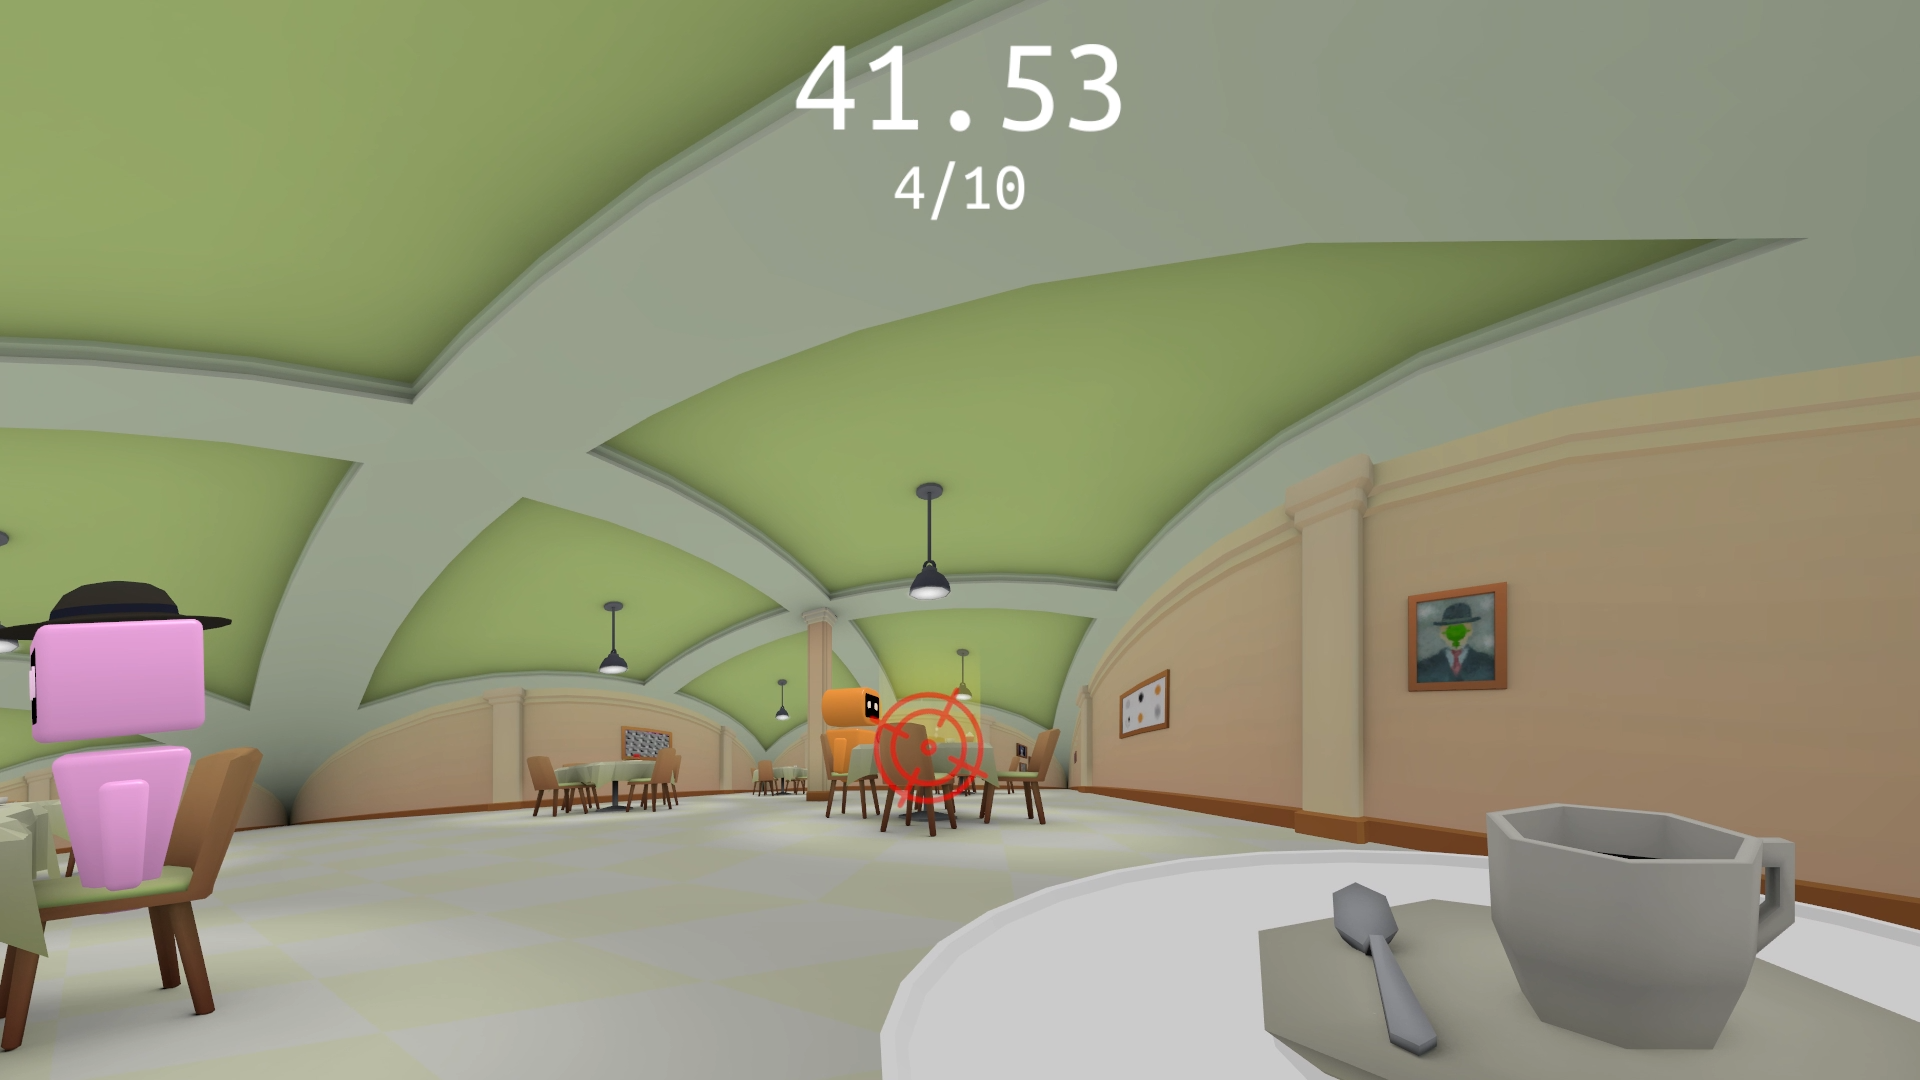
\includegraphics[width=0.75\textwidth]{NOVAthesisFiles/Images/papers/hyperbolica.png}
     \caption{A screenshot of one of the levels from the game Hyperbolica.}
    \label{fig:hyperbolica}
 \end{figure}

The visual tool by Hart et al. \cite{Hart2017} is an example on this interest, as they aimed to create a \gls{VR} experience that allows users to 
more intuitively grasp Hyperbolic Geometry. Various models were used to simulate this space, and the application permitted users to navigate through 
the \gls{VE}, which proved a challenge. Due to the space's negative curvature, phenomena like \textit{holonomy} - 
a result of parallel transporting vectors along a closed loop - occurs, which can make Hyperbolic Spaces highly disorienting, 
since it translates into effects like the floor appearing to move away 
or rotate. Authors purposed methods of solving this issue, though they were recognized as artificial means that "hack" the simulation.

Rebelo et al. \cite{Rebelo2022} have also conduct research on the use of Hyperbolic Spaces in \gls{VR}. One of the studies conducted in this work 
pretended to examine how users would react to different mappings between virtual and physical spaces, using tangible objects on a table that users 
had to move and rotate. The four different mappings (Figure~) were either mapped by linear functions - correspondent to Euclidean Spaces - 
or Hyperbolic functions - correspondent to the Non-Euclidean Spaces - in this case the hyperbolic tangent and its inverse, morphing space so that 
the center of the table occupied more or less space, respectively. Results revealed that 
there were no significant differences in terms of efficiency between two linear and hyperbolic scenarios, and the research concluded that users 
were able to adapt do Hyperbolic Spaces quickly, going in accordance with the previously mentioned work from Hart et al. \cite{Hart2017} and 
study by Pisani et al. \cite{Pisani2019}

\begin{figure}[t]
    \centering
     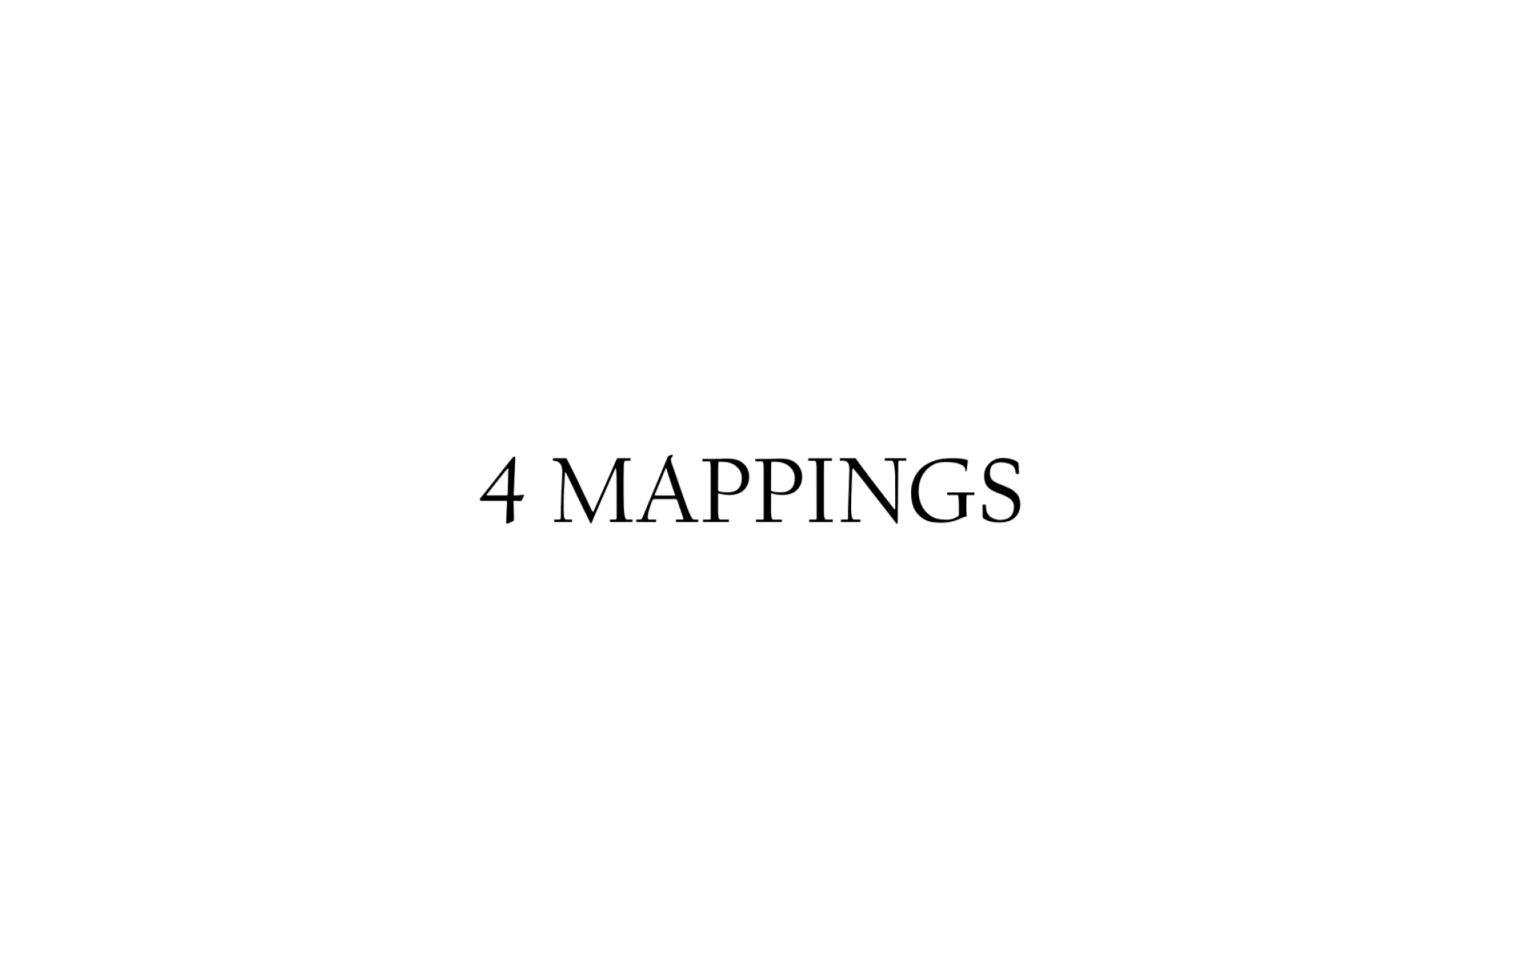
\includegraphics[width=0.75\textwidth]{NOVAthesisFiles/Images/papers/mappings.png}
     \caption{The four mappings studied by Rebelo et al. \cite{Rebelo2022}. (a) White lines represent the linear function that maps the 
     real coordinates; Blue Lines represent the linear function that maps the virtual coordinates to 3 times the size of the real table. 
     (b) is the resultant mapping of the hyperbolic tangent function (\textit{tanh}).
     (c) is the resultant mapping of the inverse hyperbolic tangent function (\textit{arctanh}). 
     [TODO: Perguntar à Rita se ainda tem estas imagens]}
    \label{fig:mappings}
 \end{figure}

 The work by Rebelo et al. \cite{Rebelo2022} additionally mentions the existance of a gap in research on the use of Hyperbolic Spaces in \gls{VR} applications, which 
 is arguably still felt, particularly on the navigation of \glspl{VE} with large interiors. Our work pretends to fill this gap, by integrating a 
 similar implementation of Hyperbolic Space mapping to test the feasibility of using these Non-Euclidean Spaces for Navigation in \gls{VR}.

\section{Procedural Content Generation}
\label{sec:pcg}

[TODO]
